\documentclass[10pt,
% a4paper,
%twocolumn,
fleqn,
%landscape, 
% papersize,
dvipdfmx,
uplatex
]{jsarticle}



\def\maru#1{\textcircled{\scriptsize#1}}%丸囲み番号

% \RequirePackage[2020/09/30]{platexrelease}

%太字設定
\usepackage[deluxe]{otf}

\usepackage{emathEy}

\usepackage[g]{esvect}

%大きな文字
\usepackage{fix-cm}

%定理環境
\usepackage{emathThm}
%\theoremstyle{boxed}
\theorembodyfont{\normalfont}
\newtheorem{Question}{問題}[subsection]
\newtheorem{Q}{}[subsection]
\newtheorem{question}[Question]{}
\newtheorem{quuestion}{}[subsection]

%セクション,大問番号のデザイン
\renewcommand{\labelenumi}{(\arabic{enumi})}
\renewcommand{\theenumii}{\alph{enumii})}
\renewcommand{\thesection}{第\arabic{section}章}

%用紙サイズの詳細設定
\usepackage{bxpapersize}
\papersizesetup{size={80mm,45mm}}
\usepackage[top=0.7zw,bottom=0truemm,left=3truemm,right=133truemm]{geometry}
\usepackage[dvipdfmx]{graphicx}

%余白など
\usepackage{setspace} % 行間
\setlength{\mathindent}{1zw}
\setlength\parindent{0pt}


%色カラーに関する設定
\usepackage{color}
\definecolor{shiro}{rgb}{0.95703125,0.87109375,0.7421875}
\definecolor{kin}{rgb}{0.95703125,0.87109375,0.7421875}
\definecolor{orange}{rgb}{1,0.7,0.2}
\definecolor{bradorange}{rgb}{1,0.5,0}
\definecolor{pink}{rgb}{0.9176,0.5686,0.5960}
\definecolor{mizu}{rgb}{0.6156,0.8,0.9955}
\color{kin}
% \pagecolor{hukamido}

\usepackage{at}%図の配置
% \usepackage{wallpaper}

\begin{document}



\at(0cm,0cm){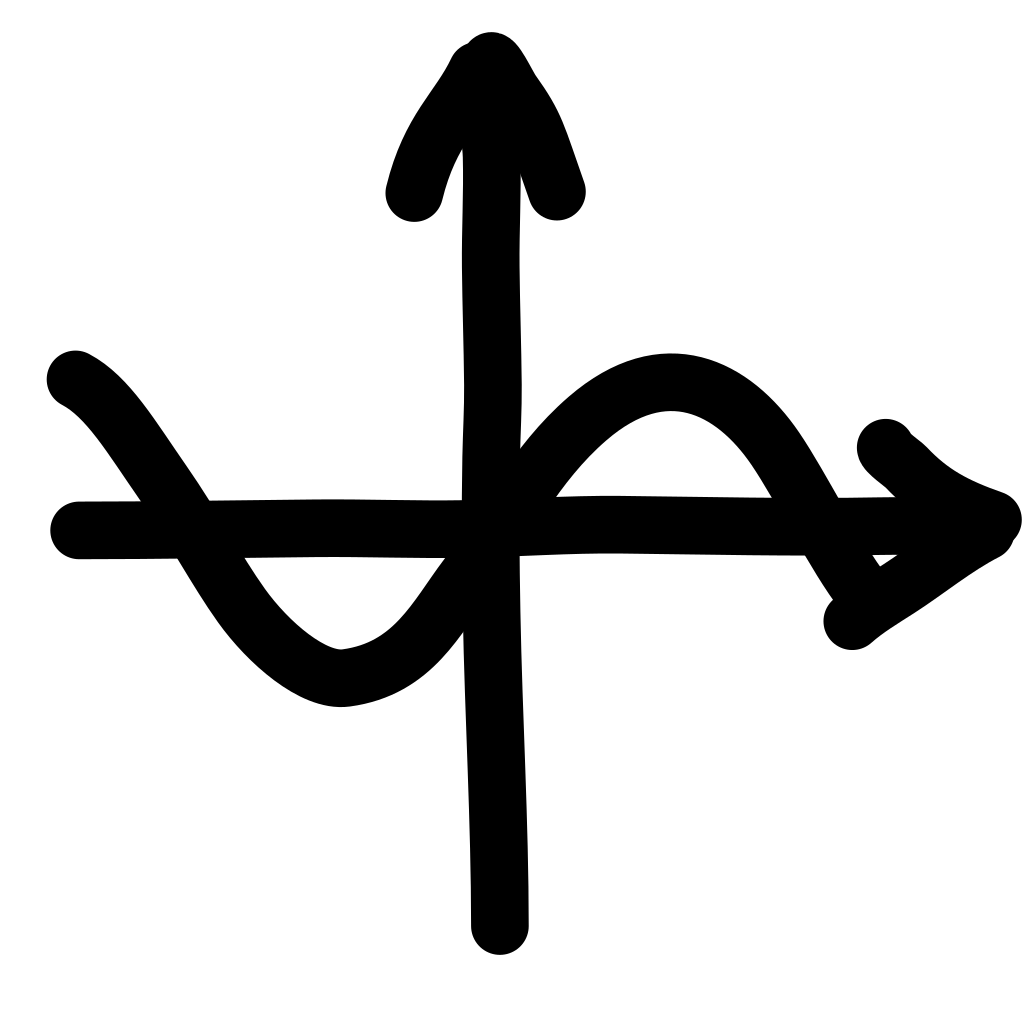
\includegraphics[width=8cm,bb=0 0 1920 1080]{./youtube/thumbnails/templates/smart_background/三角関数.jpeg}}
{\color{orange}\bf\boldmath\LARGE\underline{三角関数の方程式 Lv.1}}\vspace{0.3zw}

\normalsize
\bf\boldmath 問.$0\leqq \theta <2\pi$のとき,次の方程式を解け.

\LARGE
(1)  $2\sin \theta -1=0$\\
(2)  $2\cos \theta +\sqrt 3=0$\\
(3)  $\tan \theta =\sqrt 3$\\

\at(7.0cm,0.2cm){\small\color{bradorange}$\overset{\text{三角関数}}{\text{典型}}$}


\newpage



\at(0cm,0cm){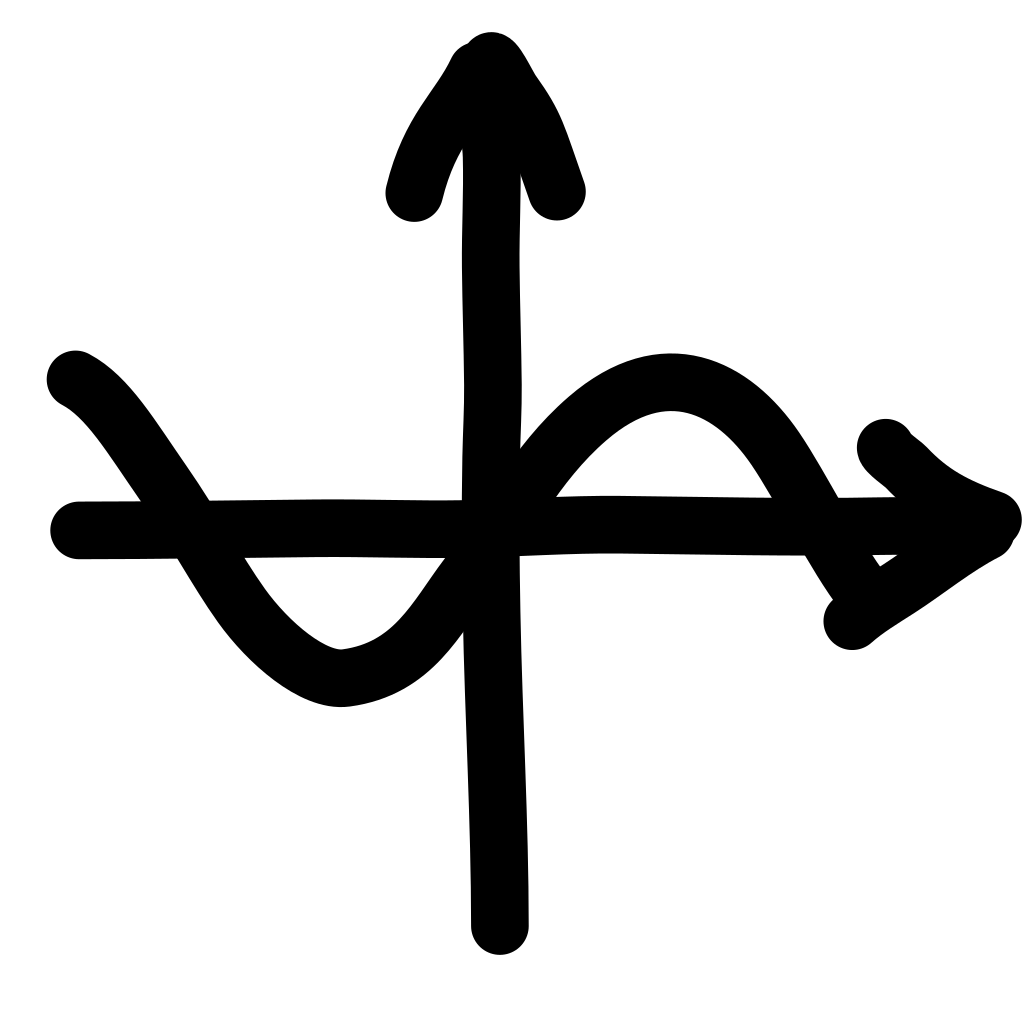
\includegraphics[width=8cm,bb=0 0 1920 1080]{./youtube/thumbnails/templates/smart_background/三角関数.jpeg}}
{\color{orange}\bf\boldmath\LARGE\underline{三角関数の不等式 Lv.1}}\vspace{0.3zw}

\normalsize
\bf\boldmath 問.$0\leqq \theta <2\pi$のとき,次の不等式を解け.

\LARGE
\vspace{-0.1zw}
(1)  $2\sin \theta <-1$\\
(2)  $\sqrt 2\cos \theta -1\geqq 0$\\
(3)  $\tan \theta \geqq 1$\\

\at(7.0cm,0.2cm){\small\color{bradorange}$\overset{\text{三角関数}}{\text{典型}}$}


\newpage



\at(0cm,0cm){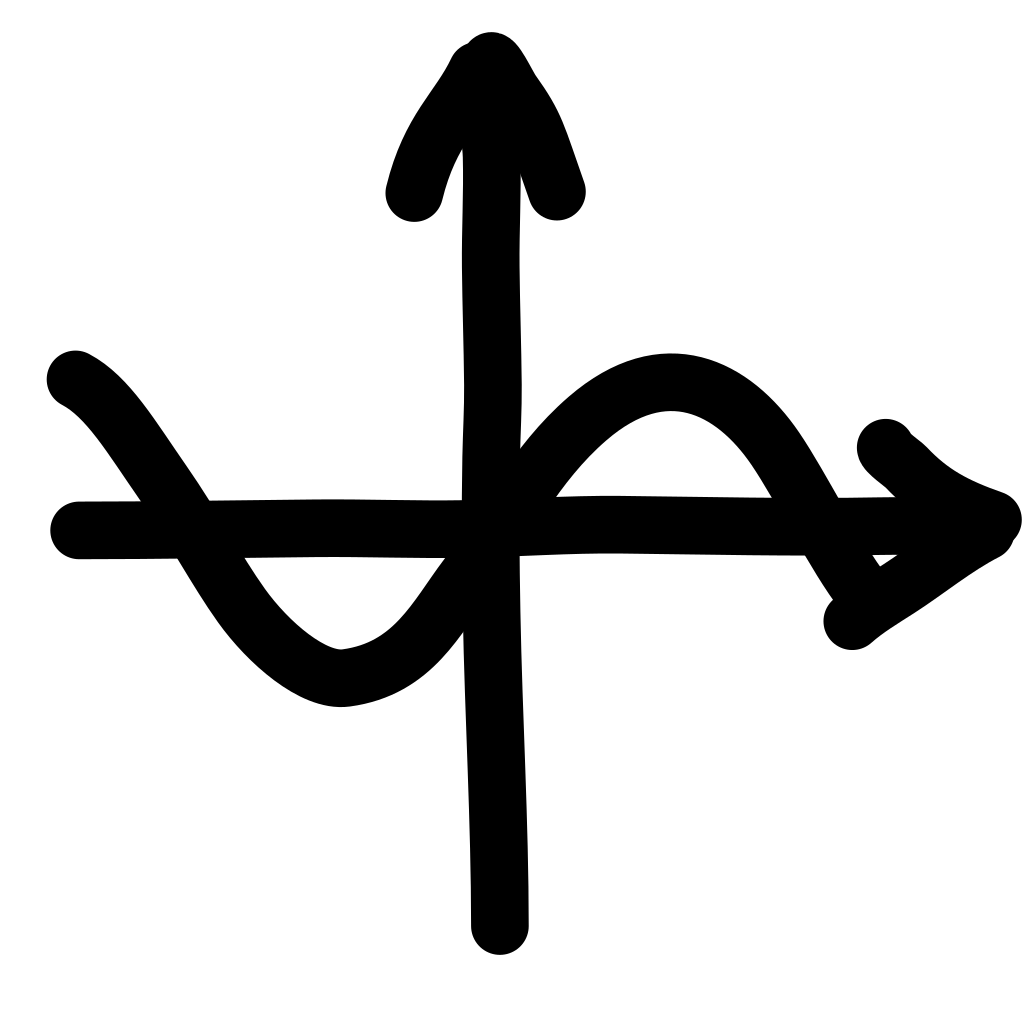
\includegraphics[width=8cm,bb=0 0 1920 1080]{./youtube/thumbnails/templates/smart_background/三角関数.jpeg}}
{\color{orange}\bf\boldmath\Large\underline{$\sin \theta$と$\cos \theta$の対称式 Lv.2}}\vspace{0.1zw}

\normalsize 
\bf\boldmath 問.$\theta$の動径が第$3$象限にあり、$\sin \theta \cos \theta =\bunsuu{1}{4}$のとき、次の式の値を求めよ.

\Large
\vspace{-0.1zw}
(1)  $\sin \theta +\cos \theta$\vspace{-0.1zw}\\
(2)  $\sin \theta -\cos \theta$\vspace{-0.1zw}\\
(3)  $\sin \theta ,\;\cos \theta$\\

\at(7.0cm,0.2cm){\small\color{bradorange}$\overset{\text{三角関数}}{\text{典型}}$}


\newpage



\at(0cm,0cm){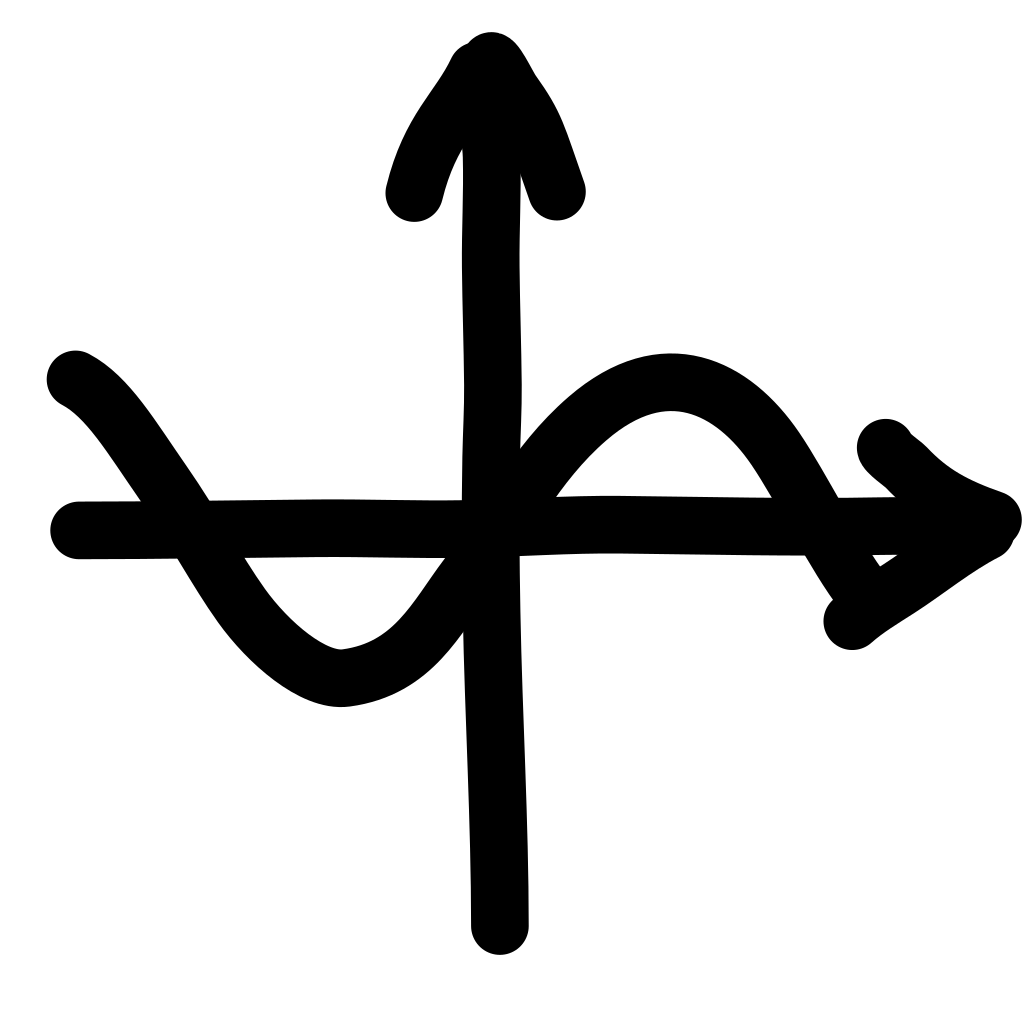
\includegraphics[width=8cm,bb=0 0 1920 1080]{./youtube/thumbnails/templates/smart_background/三角関数.jpeg}}
{\color{orange}\bf\boldmath\Large\underline{$\sin \theta$と$\cos \theta$の対称式 Lv.1}}\vspace{0.3zw}

\normalsize
\bf\boldmath 問.$\sin \theta +\cos \theta =\bunsuu{1}{2}$のとき次の値を求めよ.

\huge
\vspace{0.2zw}
(1)  $\sin \theta \cos \theta$\\
(2)  $\sin ^3\theta +\cos ^3\theta$\\

\at(7.0cm,0.2cm){\small\color{bradorange}$\overset{\text{三角関数}}{\text{典型}}$}


\newpage

\at(0cm,0cm){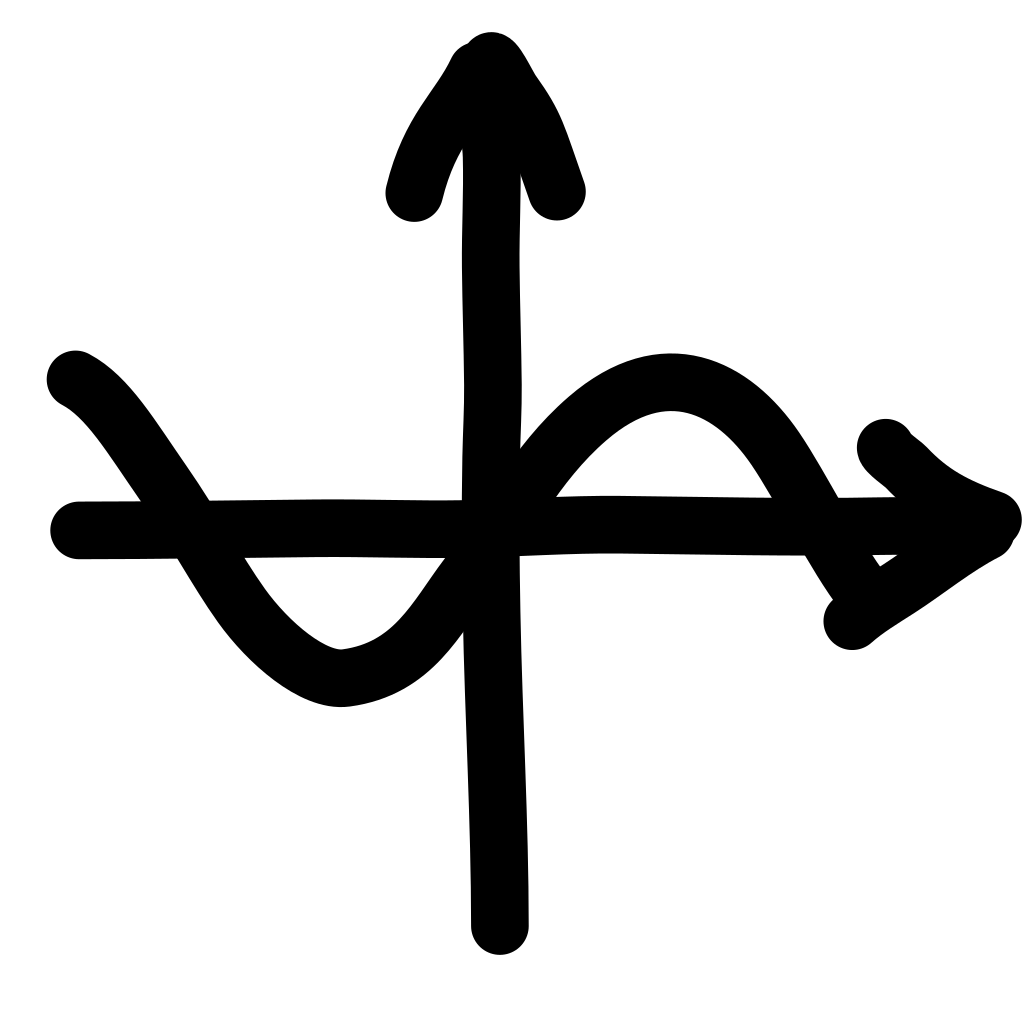
\includegraphics[width=8cm,bb=0 0 1920 1080]{./youtube/thumbnails/templates/smart_background/三角関数.jpeg}}
{\color{orange}\bf\boldmath\Large\underline{三角関数の最大$〜$合成$〜$}}\vspace{0.3zw}\\
\large 
\bf\boldmath 問.次の関数の最大値と最小値\\
\hfill およびそのときの$x$の値を求めよ.

\huge
\hspace{0.2zw} $y=\sin x+\cos x$\\ 
\hfill $\left(0\leqq x\leqq \pi \right)$
\at(7cm,0.2cm){\small\color{bradorange}$\overset{\text{三角関数}}{\text{典型}}$}

\newpage

\at(0cm,0cm){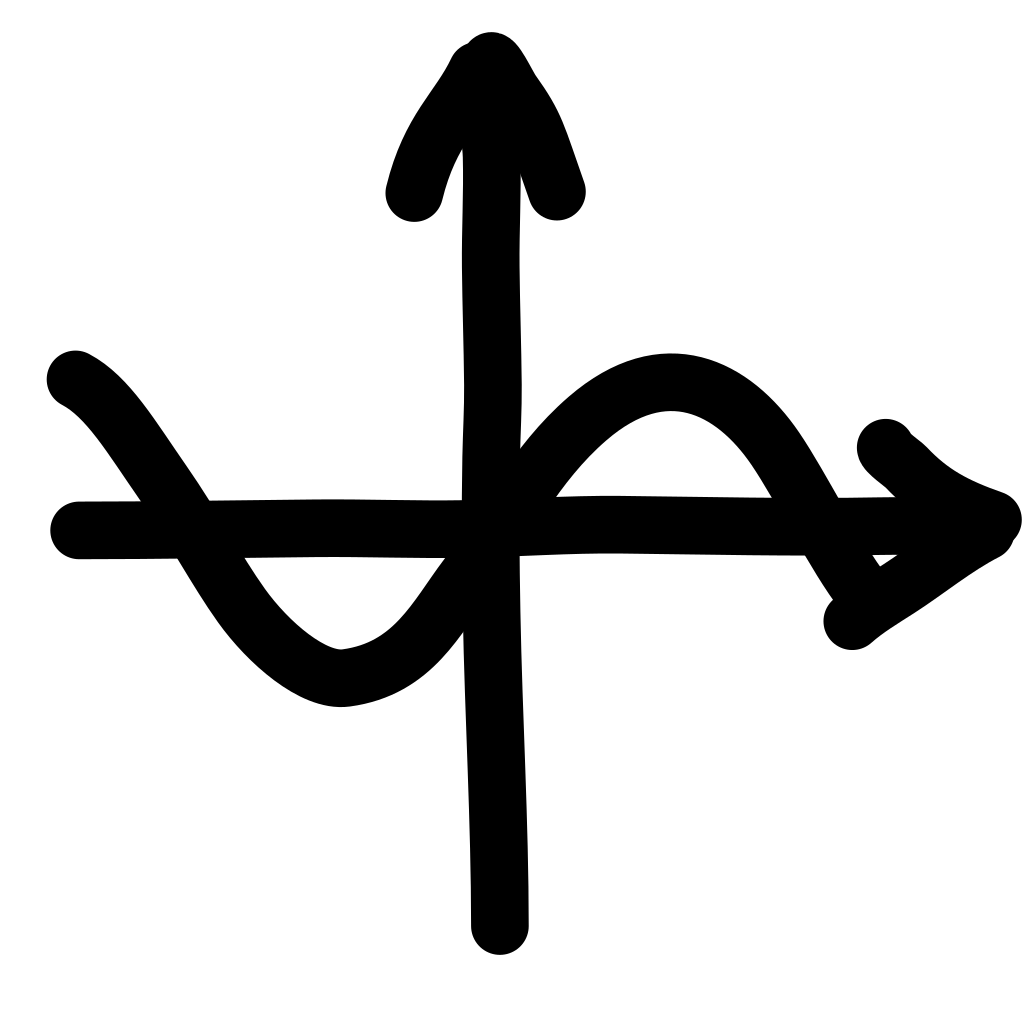
\includegraphics[width=8cm,bb=0 0 1920 1080]{./youtube/thumbnails/templates/smart_background/三角関数.jpeg}}
{\color{orange}\bf\boldmath\Large\underline{三角方程式$\cdot$不等式$〜$合成$〜$}}\vspace{0.3zw}\\
\large
\bf\boldmath 問.$0\leqq x<2\pi$のとき,\\
\hfill 次の方程式$\cdot$不等式を解け.

\LARGE
(1)  $\sin x-\sqrt 3\cos x=1$\\
(2)  $\sin x-\sqrt 3\cos x>1$\\

\at(7cm,0.2cm){\small\color{bradorange}$\overset{\text{三角関数}}{\text{典型}}$}

\newpage

\at(0cm,0cm){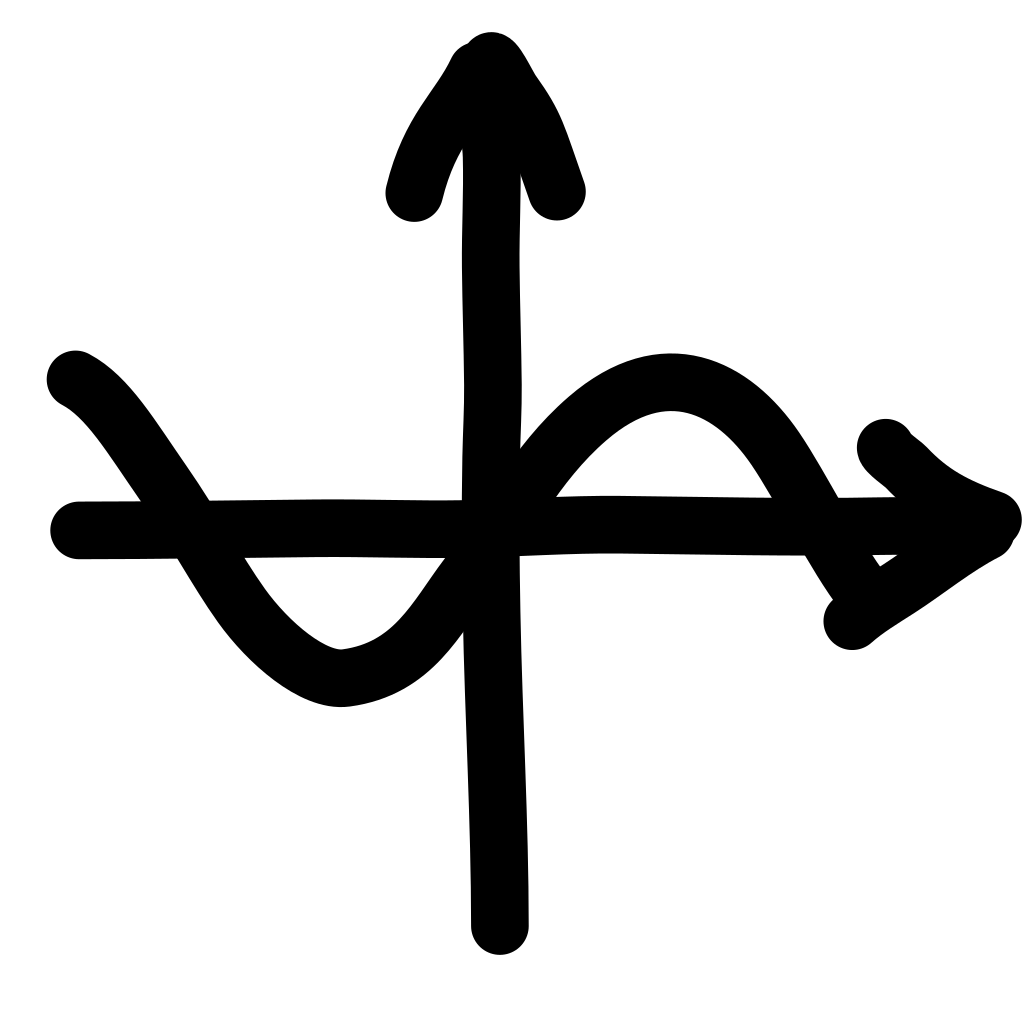
\includegraphics[width=8cm,bb=0 0 1920 1080]{./youtube/thumbnails/templates/smart_background/三角関数.jpeg}}
{\color{orange}\bf\boldmath\Large\underline{$2$倍角を含む方程式$\cdot$不等式}}\vspace{0.3zw}\\
\large 
\bf\boldmath 問.$0\leqq x<2\pi$のとき,\\
\hfill 次の方程式$\cdot$不等式を解け.

\LARGE
(1)  $\sin 2x=\sin x$\\
(2)  $\cos 2\theta \leqq 3\sin x-1$\\

\at(7cm,0.2cm){\small\color{bradorange}$\overset{\text{三角関数}}{\text{典型}}$}

\newpage

\at(0cm,0cm){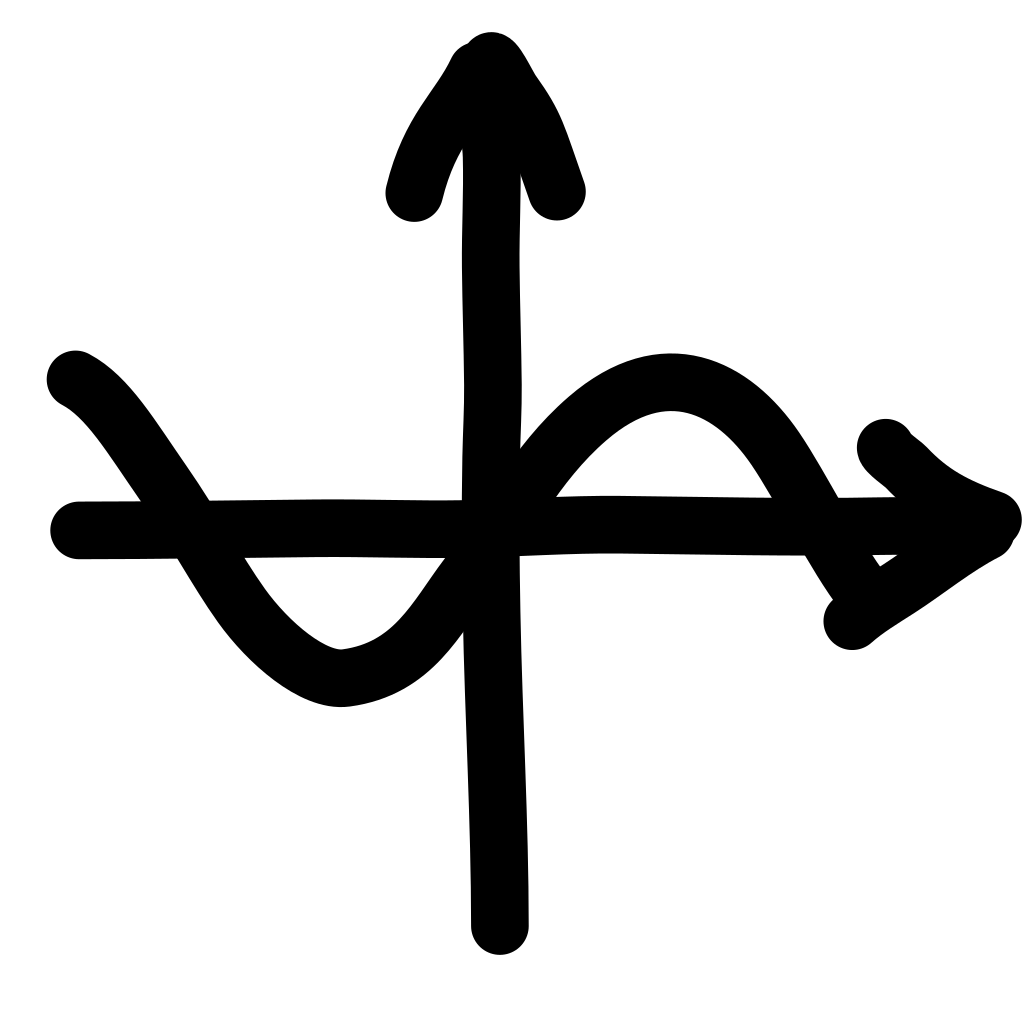
\includegraphics[width=8cm,bb=0 0 1920 1080]{./youtube/thumbnails/templates/smart_background/三角関数.jpeg}}
{\color{orange}\bf\boldmath\LARGE\underline{$2$直線のなす鋭角$\theta$}}\vspace{0.3zw}\\
\LARGE 
\bf\boldmath 問.$2$直線$\left\{\begin{array}{l}y=3x-1,\;\\y=\bunsuu{1}{2}x+1\end{array}\right.$\vspace{0.3zw}\\
\hfill のなす鋭角$\theta$を求めよ.
\at(7cm,0.2cm){\small\color{bradorange}$\overset{\text{三角関数}}{\text{典型}}$}

\newpage

\at(0cm,0cm){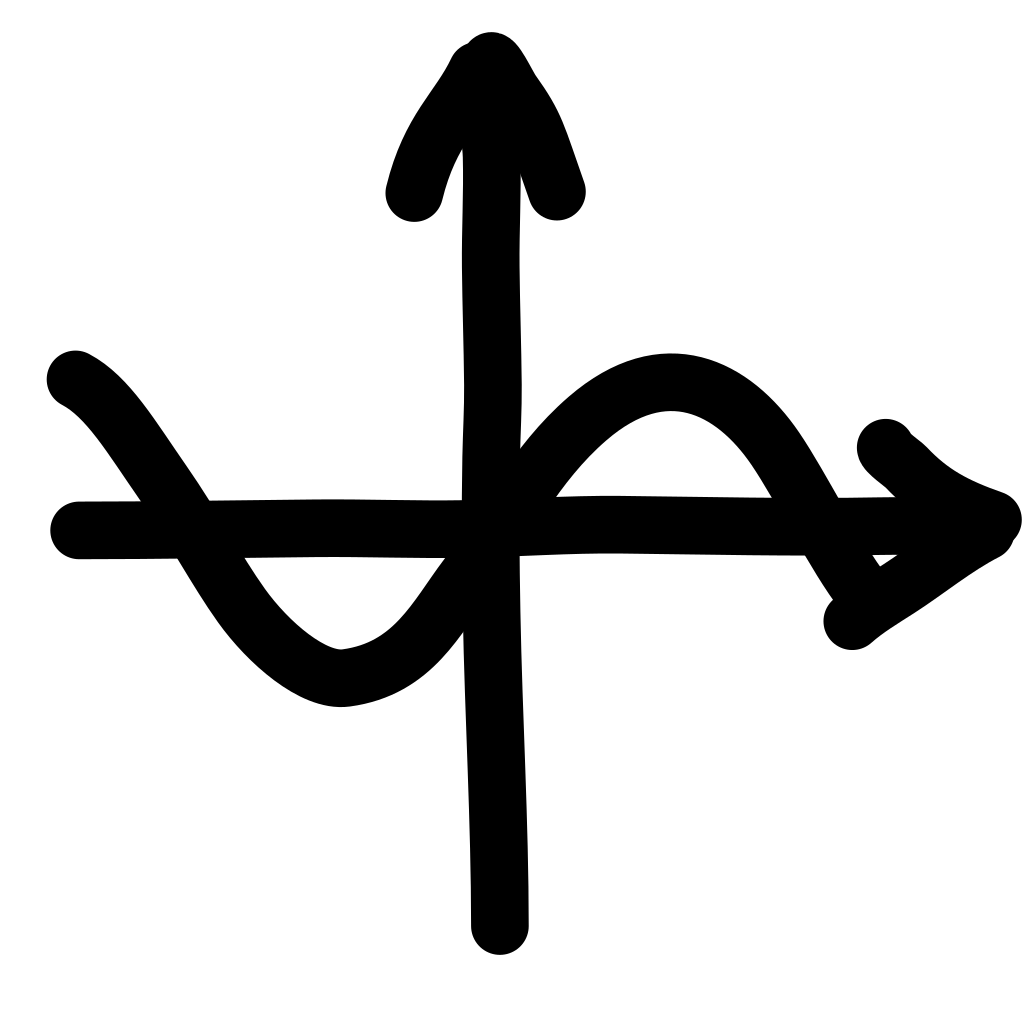
\includegraphics[width=8cm,bb=0 0 1920 1080]{./youtube/thumbnails/templates/smart_background/三角関数.jpeg}}
{\color{orange}\bf\boldmath\Large\underline{$2$次関数の最大最小に帰着}}\vspace{0.3zw}

\large 
\bf\boldmath 問.$0\leqq \theta <2\pi$のとき,関数

\Huge
\hspace{0.1zw}
$y=\sin ^2\theta -\cos \theta$

\large 
\vspace{0.8zw}
の最大値と最小値を求めよ.\\
\hfill また,そのときの$\theta$の値を求めよ.
\at(7cm,0.2cm){\small\color{bradorange}$\overset{\text{三角関数}}{\text{典型}}$}

\newpage

\at(0cm,0cm){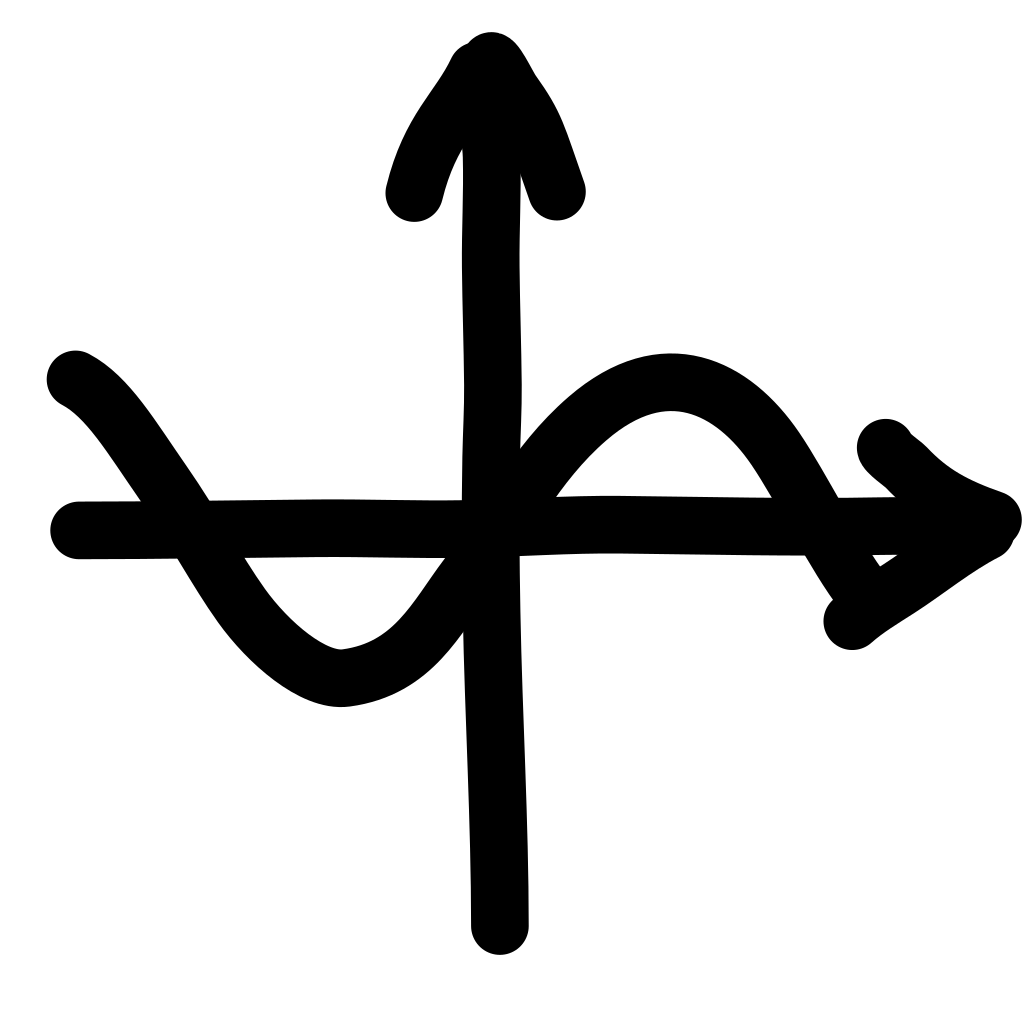
\includegraphics[width=8cm,bb=0 0 1920 1080]{./youtube/thumbnails/templates/smart_background/三角関数.jpeg}}
{\color{orange}\bf\boldmath\normalsize\underline{三角方程式$\cdot$不等式$〜2$次方程式に帰着$〜$}}\vspace{0.3zw}

\large 
\bf\boldmath 問.$0\leqq \theta <2\pi$のとき,\\
\hfill 次の方程式$\cdot$不等式を解け.

\LARGE
(1)  $2\sin ^2\theta +\cos \theta -2=0$\\
(2)  $2\cos ^2\theta \leqq 3\sin \theta$\\

\at(7cm,0.2cm){\small\color{bradorange}$\overset{\text{三角関数}}{\text{典型}}$}

\newpage

\at(0cm,0cm){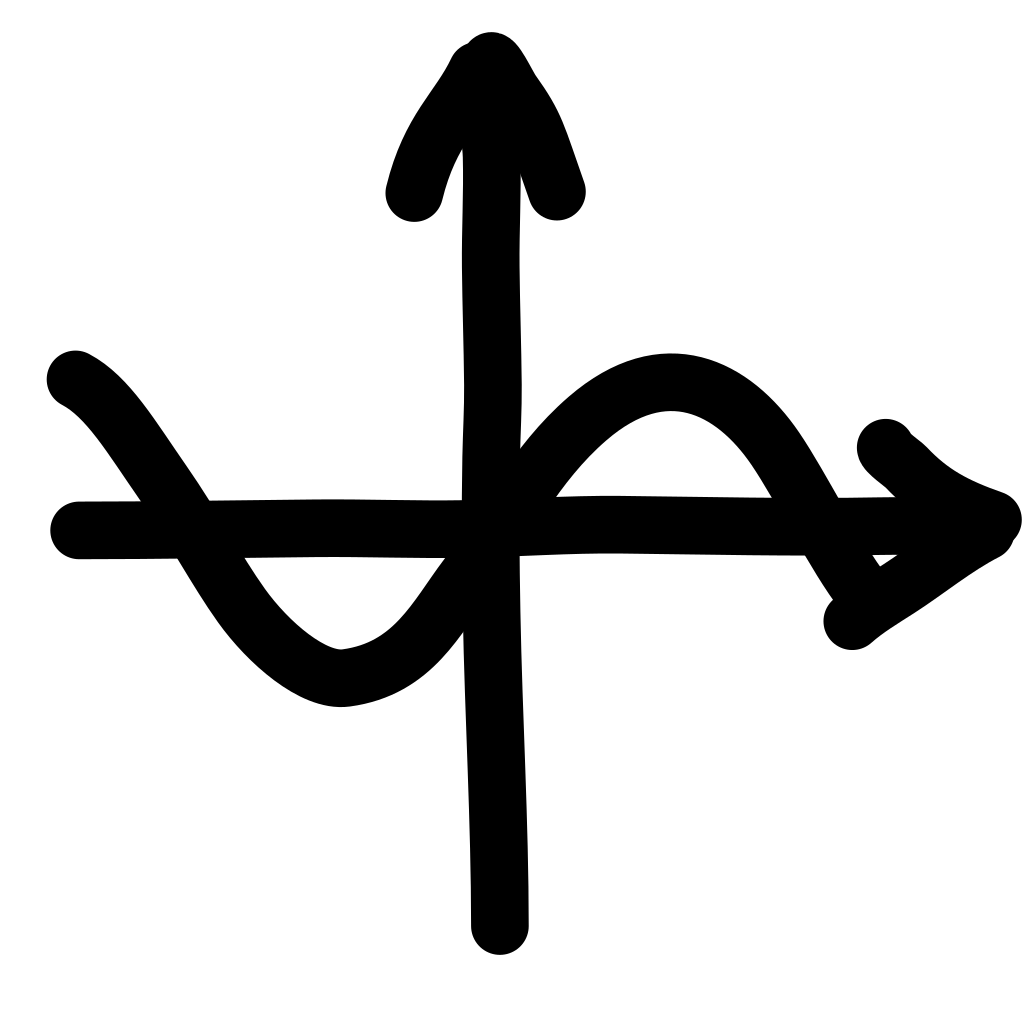
\includegraphics[width=8cm,bb=0 0 1920 1080]{./youtube/thumbnails/templates/smart_background/三角関数.jpeg}}
{\color{orange}\bf\boldmath\Large\underline{三角方程式$\cdot$不等式$〜$中級$〜$}}\vspace{0.3zw}\\
\small 
\bf\boldmath 問.$0\leqq \theta <2\pi$のとき,次の方程式$\cdot$不等式を解け.\vspace{0.5zw}

\Large 
(1)  $\sin \left(2\theta -\bunsuu{\pi }{3}\right)=\bunsuu{{\sqrt 3}}{2}$\\
(2)  $\sin \left(2\theta -\bunsuu{\pi }{3}\right)\leqq \bunsuu{{\sqrt 3}}{2}$\\

\at(7cm,0.2cm){\small\color{bradorange}$\overset{\text{三角関数}}{\text{典型}}$}

\newpage

\at(0cm,0cm){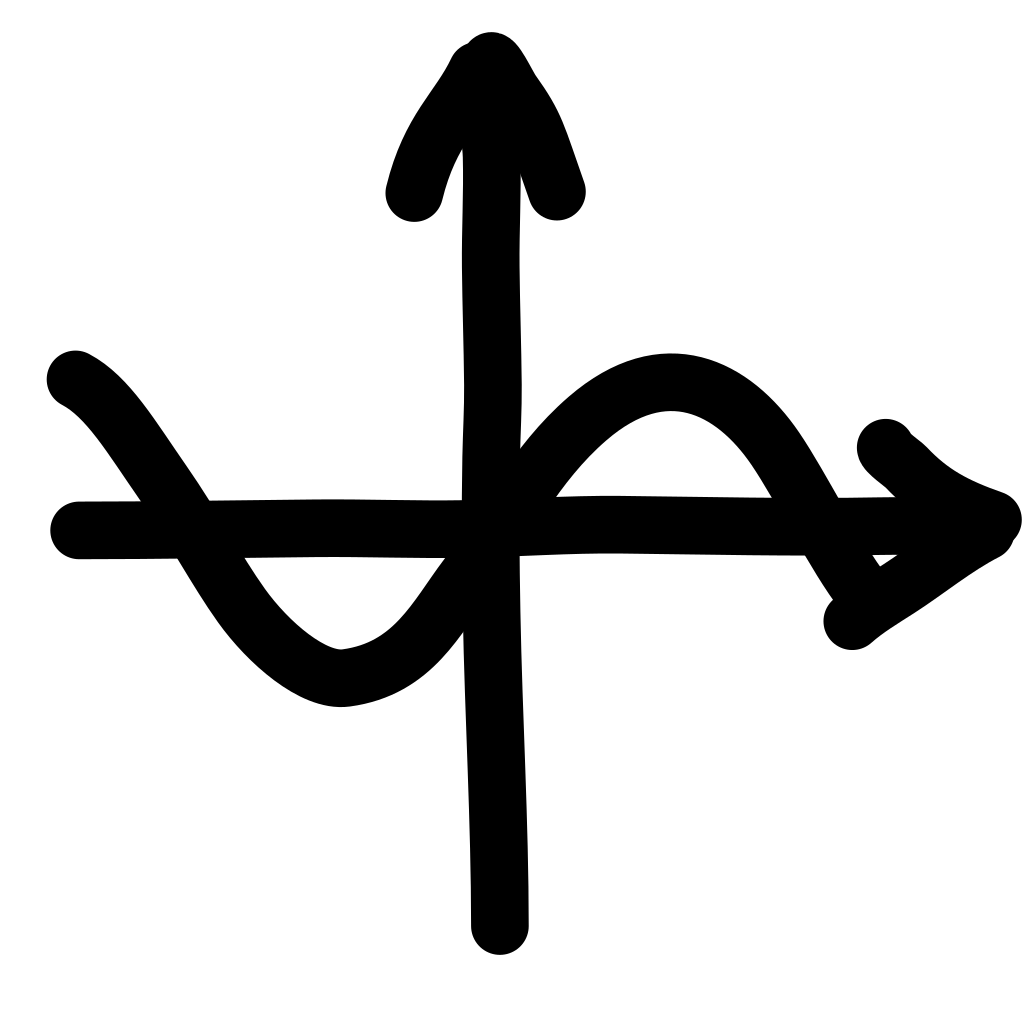
\includegraphics[width=8cm,bb=0 0 1920 1080]{./youtube/thumbnails/templates/smart_background/三角関数.jpeg}}
{\color{orange}\bf\boldmath\LARGE\underline{三角関数の相互関係}}\vspace{0.3zw}

\huge
\bf\boldmath 問.$\tan \theta =3$のとき,

\Huge
\hspace{0.2zw} $\sin \theta ,\;\cos \theta$の値 \hfill \hspace{0.2zw}

\huge
\hfill を求めよ.\\

\at(7cm,0.2cm){\small\color{bradorange}$\overset{\text{三角関数}}{\text{典型}}$}



\end{document}

